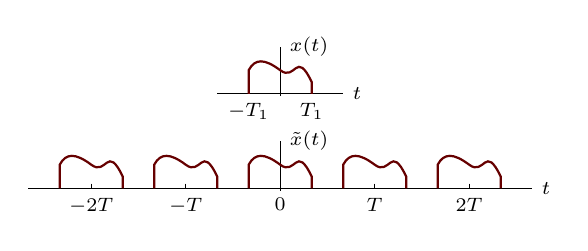
\begin{tikzpicture}[every node/.style={font=\scriptsize}, x=0.4cm, y=0.3cm]
	\def\T1{1cm}		
	\def\T{3}
	\draw (-2, 0) -- (2,0)  node [anchor=west] {$t$};
	\draw (0, -0.1) -- (0, 2) node [anchor=west] {$x(t)$};
	\def\pulse{

		--++(0,1) .. controls ++(0.2,0.5) and ++(-0.5,0.5) .. ++(1,0) .. controls ++(0.5,-0.5) and ++(-0.5,1.4) .. ++(1,-0.5) -- ++(0,-0.5)
	}
	\draw[thick, red!40!black] (-1,0) \pulse;
	\node at (-1,0) [anchor=north] {$-T_1$};
	\node at (1,0) [anchor=north] {$T_1$};
	
	\begin{scope}[yshift = -1.2cm]
		\draw (-8, 0) -- (8,0)  node [anchor=west] {$t$};
		\draw (0, -0.1) -- (0, 2) node [anchor=west] {$\tilde{x}(t)$};	
		\foreach \x/\l in {-2/-2T, -1/-T, 0/0, 1/T, 2/2T}	
		{
			\draw[thick, red!40!black] (\x*\T -1, 0) \pulse;
			\draw (\x*\T, 0.2) -- ++(0, -0.2) node [anchor=north] {$\l$};
		}		
	
	\end{scope}
	
\end{tikzpicture} 